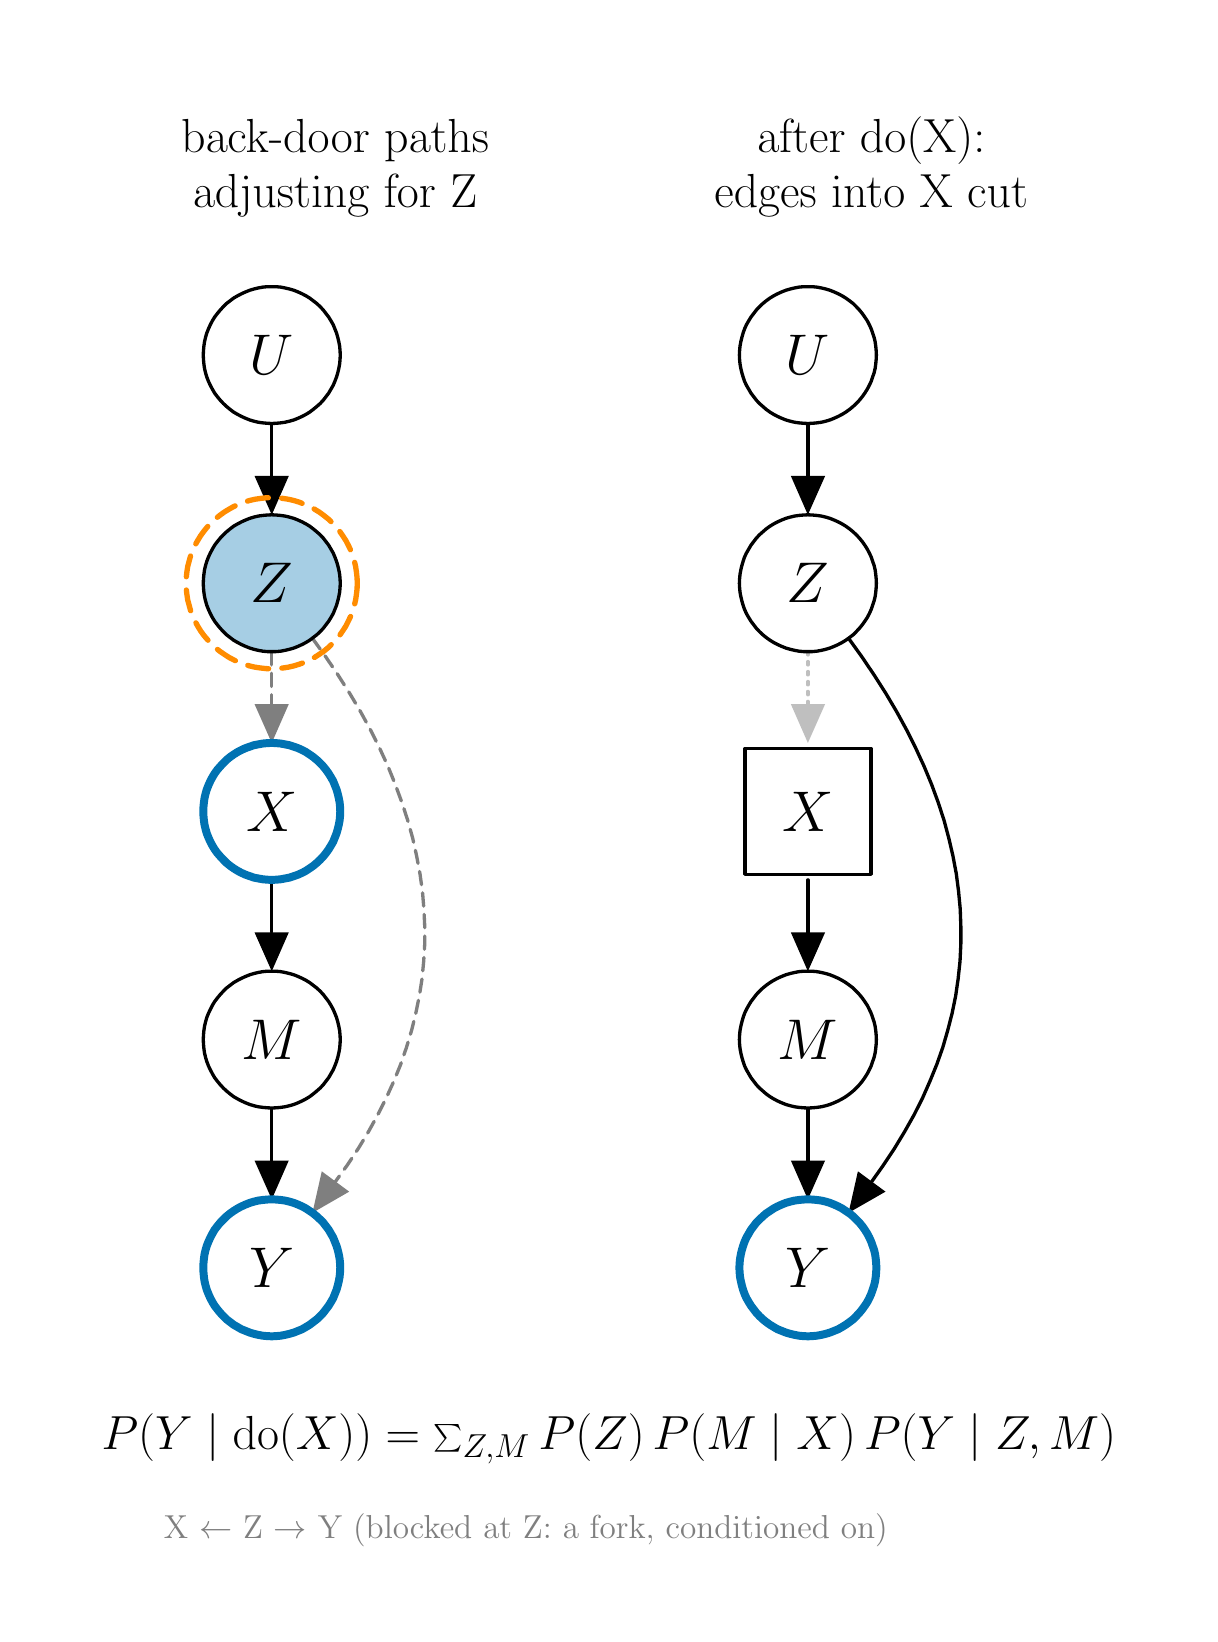
\begin{tikzpicture}[x=0.75pt,y=-0.75pt,every node/.style={inner sep=0pt,outer sep=0pt},font=\fontsize{9}{10.8}\selectfont]
\definecolor{pbp1}{RGB}{255,255,255}
\definecolor{pbp2}{RGB}{0,0,0}
\definecolor{pbp3}{RGB}{127,127,127}
\definecolor{pbp4}{RGB}{166,206,228}
\definecolor{pbp5}{RGB}{255,140,0}
\definecolor{pbp6}{RGB}{0,114,178}
\definecolor{pbp7}{RGB}{191,191,191}
\useasboundingbox (0,0) rectangle (560,764);
\path[fill=pbp1] (0,0) rectangle (560,764);
\begin{scope}
\clip (10,10.4) rectangle (550,753.6);
\path[draw=pbp2,line width=1.2pt,line join=round,line cap=round] (117.6,190.7) -- (117.6,216);
\path[fill=pbp2] (117.6,234.7) -- (125.8,216) -- (109.3,216) -- cycle;
\path[draw=pbp3,line width=1.2pt,dash pattern=on 4.8pt off 3pt,line join=round,line cap=round] (117.6,300.6) -- (117.6,325.9);
\path[fill=pbp3] (117.6,344.6) -- (125.8,325.9) -- (109.3,325.9) -- cycle;
\path[draw=pbp3,line width=1.2pt,dash pattern=on 4.8pt off 3pt,line join=round,line cap=round] (137.2,294.2) -- (143.6,303.1) -- (149.6,312) -- (155.2,320.8) -- (160.4,329.6) -- (165.2,338.4) -- (169.6,347.2) -- (173.6,355.9) -- (177.1,364.6) -- (180.3,373.3) -- (183.1,381.9) -- (185.5,390.5) -- (187.4,399.1) -- (189,407.6) -- (190.2,416.1) -- (190.9,424.6) -- (191.3,433) -- (191.3,441.4) -- (190.8,449.8) -- (190,458.2) -- (188.7,466.5) -- (187,474.8) -- (185,483) -- (182.5,491.3) -- (179.7,499.5) -- (176.4,507.6) -- (172.7,515.8) -- (168.6,523.9) -- (164.2,531.9) -- (159.3,540) -- (154,548) -- (148.3,555.9);
\path[fill=pbp3] (137.2,571) -- (154.9,560.8) -- (141.7,551) -- cycle;
\path[draw=pbp2,line width=1.2pt,line join=round,line cap=round] (117.6,520.5) -- (117.6,545.8);
\path[fill=pbp2] (117.6,564.5) -- (125.8,545.8) -- (109.3,545.8) -- cycle;
\path[draw=pbp2,line width=1.2pt,line join=round,line cap=round] (117.6,410.6) -- (117.6,435.9);
\path[fill=pbp2] (117.6,454.6) -- (125.8,435.9) -- (109.3,435.9) -- cycle;
\path[fill=pbp1,draw=pbp2,line width=1.2pt,line join=round,line cap=round] (150.6,157.7) -- (150.5,155.6) -- (150.3,153.4) -- (149.9,151.3) -- (149.4,149.2) -- (148.8,147.1) -- (148,145.1) -- (147.2,143.1) -- (146.1,141.2) -- (145,139.4) -- (143.7,137.7) -- (142.4,136) -- (140.9,134.4) -- (139.3,132.9) -- (137.6,131.6) -- (135.9,130.3) -- (134.1,129.2) -- (132.2,128.2) -- (130.2,127.3) -- (128.2,126.5) -- (126.1,125.9) -- (124,125.4) -- (121.9,125) -- (119.7,124.8) -- (117.6,124.8) -- (115.4,124.8) -- (113.3,125) -- (111.1,125.4) -- (109,125.9) -- (107,126.5) -- (105,127.3) -- (103,128.2) -- (101.1,129.2) -- (99.2,130.3) -- (97.5,131.6) -- (95.8,132.9) -- (94.3,134.4) -- (92.8,136) -- (91.4,137.7) -- (90.1,139.4) -- (89,141.2) -- (88,143.1) -- (87.1,145.1) -- (86.3,147.1) -- (85.7,149.2) -- (85.2,151.3) -- (84.9,153.4) -- (84.7,155.6) -- (84.6,157.7) -- (84.7,159.9) -- (84.9,162) -- (85.2,164.2) -- (85.7,166.3) -- (86.3,168.3) -- (87.1,170.4) -- (88,172.3) -- (89,174.2) -- (90.1,176.1) -- (91.4,177.8) -- (92.8,179.5) -- (94.3,181.1) -- (95.8,182.5) -- (97.5,183.9) -- (99.2,185.2) -- (101.1,186.3) -- (103,187.3) -- (105,188.2) -- (107,189) -- (109,189.6) -- (111.1,190.1) -- (113.3,190.4) -- (115.4,190.6) -- (117.6,190.7) -- (119.7,190.6) -- (121.9,190.4) -- (124,190.1) -- (126.1,189.6) -- (128.2,189) -- (130.2,188.2) -- (132.2,187.3) -- (134.1,186.3) -- (135.9,185.2) -- (137.6,183.9) -- (139.3,182.5) -- (140.9,181.1) -- (142.4,179.5) -- (143.7,177.8) -- (145,176.1) -- (146.1,174.2) -- (147.2,172.3) -- (148,170.4) -- (148.8,168.3) -- (149.4,166.3) -- (149.9,164.2) -- (150.3,162) -- (150.5,159.9) -- cycle;
\node[anchor=center,font=\fontsize{19.788}{23.746}\selectfont] at (117.6,157.7) {$U$};
\path[fill=pbp4,draw=pbp2,line width=1.2pt,line join=round,line cap=round] (150.6,267.7) -- (150.5,265.5) -- (150.3,263.4) -- (149.9,261.2) -- (149.4,259.1) -- (148.8,257.1) -- (148,255) -- (147.2,253.1) -- (146.1,251.2) -- (145,249.3) -- (143.7,247.6) -- (142.4,245.9) -- (140.9,244.3) -- (139.3,242.9) -- (137.6,241.5) -- (135.9,240.2) -- (134.1,239.1) -- (132.2,238.1) -- (130.2,237.2) -- (128.2,236.4) -- (126.1,235.8) -- (124,235.3) -- (121.9,235) -- (119.7,234.8) -- (117.6,234.7) -- (115.4,234.8) -- (113.3,235) -- (111.1,235.3) -- (109,235.8) -- (107,236.4) -- (105,237.2) -- (103,238.1) -- (101.1,239.1) -- (99.2,240.2) -- (97.5,241.5) -- (95.8,242.9) -- (94.3,244.3) -- (92.8,245.9) -- (91.4,247.6) -- (90.1,249.3) -- (89,251.2) -- (88,253.1) -- (87.1,255) -- (86.3,257.1) -- (85.7,259.1) -- (85.2,261.2) -- (84.9,263.4) -- (84.7,265.5) -- (84.6,267.7) -- (84.7,269.8) -- (84.9,272) -- (85.2,274.1) -- (85.7,276.2) -- (86.3,278.3) -- (87.1,280.3) -- (88,282.3) -- (89,284.2) -- (90.1,286) -- (91.4,287.7) -- (92.8,289.4) -- (94.3,291) -- (95.8,292.5) -- (97.5,293.8) -- (99.2,295.1) -- (101.1,296.2) -- (103,297.2) -- (105,298.1) -- (107,298.9) -- (109,299.5) -- (111.1,300) -- (113.3,300.4) -- (115.4,300.6) -- (117.6,300.6) -- (119.7,300.6) -- (121.9,300.4) -- (124,300) -- (126.1,299.5) -- (128.2,298.9) -- (130.2,298.1) -- (132.2,297.2) -- (134.1,296.2) -- (135.9,295.1) -- (137.6,293.8) -- (139.3,292.5) -- (140.9,291) -- (142.4,289.4) -- (143.7,287.7) -- (145,286) -- (146.1,284.2) -- (147.2,282.3) -- (148,280.3) -- (148.8,278.3) -- (149.4,276.2) -- (149.9,274.1) -- (150.3,272) -- (150.5,269.8) -- cycle;
\path[draw=pbp5,line width=1.92pt,dash pattern=on 7.65pt off 4.8pt,line join=round,line cap=round] (158.8,267.7) -- (158.7,265) -- (158.4,262.3) -- (158,259.6) -- (157.4,257) -- (156.6,254.4) -- (155.7,251.9) -- (154.5,249.4) -- (153.3,247.1) -- (151.8,244.8) -- (150.3,242.6) -- (148.6,240.5) -- (146.7,238.5) -- (144.8,236.7) -- (142.7,235) -- (140.5,233.4) -- (138.2,232) -- (135.8,230.7) -- (133.3,229.6) -- (130.8,228.6) -- (128.2,227.8) -- (125.6,227.2) -- (123,226.8) -- (120.3,226.5) -- (117.6,226.4) -- (114.9,226.5) -- (112.2,226.8) -- (109.5,227.2) -- (106.9,227.8) -- (104.3,228.6) -- (101.8,229.6) -- (99.3,230.7) -- (97,232) -- (94.7,233.4) -- (92.5,235) -- (90.4,236.7) -- (88.4,238.5) -- (86.6,240.5) -- (84.9,242.6) -- (83.3,244.8) -- (81.9,247.1) -- (80.6,249.4) -- (79.5,251.9) -- (78.5,254.4) -- (77.8,257) -- (77.1,259.6) -- (76.7,262.3) -- (76.4,265) -- (76.3,267.7) -- (76.4,270.4) -- (76.7,273) -- (77.1,275.7) -- (77.8,278.3) -- (78.5,280.9) -- (79.5,283.4) -- (80.6,285.9) -- (81.9,288.3) -- (83.3,290.6) -- (84.9,292.8) -- (86.6,294.8) -- (88.4,296.8) -- (90.4,298.7) -- (92.5,300.4) -- (94.7,301.9) -- (97,303.4) -- (99.3,304.6) -- (101.8,305.8) -- (104.3,306.7) -- (106.9,307.5) -- (109.5,308.1) -- (112.2,308.5) -- (114.9,308.8) -- (117.6,308.9) -- (120.3,308.8) -- (123,308.5) -- (125.6,308.1) -- (128.2,307.5) -- (130.8,306.7) -- (133.3,305.8) -- (135.8,304.6) -- (138.2,303.4) -- (140.5,301.9) -- (142.7,300.4) -- (144.8,298.7) -- (146.7,296.8) -- (148.6,294.8) -- (150.3,292.8) -- (151.8,290.6) -- (153.3,288.3) -- (154.5,285.9) -- (155.7,283.4) -- (156.6,280.9) -- (157.4,278.3) -- (158,275.7) -- (158.4,273) -- (158.7,270.4) -- (158.8,267.7);
\node[anchor=center,font=\fontsize{19.788}{23.746}\selectfont] at (117.6,267.7) {$Z$};
\path[fill=pbp1,draw=pbp6,line width=2.88pt,line join=round,line cap=round] (150.6,377.6) -- (150.5,375.4) -- (150.3,373.3) -- (149.9,371.2) -- (149.4,369.1) -- (148.8,367) -- (148,365) -- (147.2,363) -- (146.1,361.1) -- (145,359.3) -- (143.7,357.5) -- (142.4,355.9) -- (140.9,354.3) -- (139.3,352.8) -- (137.6,351.4) -- (135.9,350.2) -- (134.1,349) -- (132.2,348) -- (130.2,347.1) -- (128.2,346.4) -- (126.1,345.7) -- (124,345.3) -- (121.9,344.9) -- (119.7,344.7) -- (117.6,344.6) -- (115.4,344.7) -- (113.3,344.9) -- (111.1,345.3) -- (109,345.7) -- (107,346.4) -- (105,347.1) -- (103,348) -- (101.1,349) -- (99.2,350.2) -- (97.5,351.4) -- (95.8,352.8) -- (94.3,354.3) -- (92.8,355.9) -- (91.4,357.5) -- (90.1,359.3) -- (89,361.1) -- (88,363) -- (87.1,365) -- (86.3,367) -- (85.7,369.1) -- (85.2,371.2) -- (84.9,373.3) -- (84.7,375.4) -- (84.6,377.6) -- (84.7,379.8) -- (84.9,381.9) -- (85.2,384) -- (85.7,386.1) -- (86.3,388.2) -- (87.1,390.2) -- (88,392.2) -- (89,394.1) -- (90.1,395.9) -- (91.4,397.7) -- (92.8,399.3) -- (94.3,400.9) -- (95.8,402.4) -- (97.5,403.8) -- (99.2,405) -- (101.1,406.2) -- (103,407.2) -- (105,408.1) -- (107,408.8) -- (109,409.5) -- (111.1,409.9) -- (113.3,410.3) -- (115.4,410.5) -- (117.6,410.6) -- (119.7,410.5) -- (121.9,410.3) -- (124,409.9) -- (126.1,409.5) -- (128.2,408.8) -- (130.2,408.1) -- (132.2,407.2) -- (134.1,406.2) -- (135.9,405) -- (137.6,403.8) -- (139.3,402.4) -- (140.9,400.9) -- (142.4,399.3) -- (143.7,397.7) -- (145,395.9) -- (146.1,394.1) -- (147.2,392.2) -- (148,390.2) -- (148.8,388.2) -- (149.4,386.1) -- (149.9,384) -- (150.3,381.9) -- (150.5,379.8) -- cycle;
\node[anchor=center,font=\fontsize{19.788}{23.746}\selectfont] at (117.6,377.6) {$X$};
\path[fill=pbp1,draw=pbp6,line width=2.88pt,line join=round,line cap=round] (150.6,597.5) -- (150.5,595.3) -- (150.3,593.2) -- (149.9,591) -- (149.4,588.9) -- (148.8,586.9) -- (148,584.9) -- (147.2,582.9) -- (146.1,581) -- (145,579.1) -- (143.7,577.4) -- (142.4,575.7) -- (140.9,574.2) -- (139.3,572.7) -- (137.6,571.3) -- (135.9,570.1) -- (134.1,568.9) -- (132.2,567.9) -- (130.2,567) -- (128.2,566.2) -- (126.1,565.6) -- (124,565.1) -- (121.9,564.8) -- (119.7,564.6) -- (117.6,564.5) -- (115.4,564.6) -- (113.3,564.8) -- (111.1,565.1) -- (109,565.6) -- (107,566.2) -- (105,567) -- (103,567.9) -- (101.1,568.9) -- (99.2,570.1) -- (97.5,571.3) -- (95.8,572.7) -- (94.3,574.2) -- (92.8,575.7) -- (91.4,577.4) -- (90.1,579.1) -- (89,581) -- (88,582.9) -- (87.1,584.9) -- (86.3,586.9) -- (85.7,588.9) -- (85.2,591) -- (84.9,593.2) -- (84.7,595.3) -- (84.6,597.5) -- (84.7,599.6) -- (84.9,601.8) -- (85.2,603.9) -- (85.7,606) -- (86.3,608.1) -- (87.1,610.1) -- (88,612.1) -- (89,614) -- (90.1,615.8) -- (91.4,617.5) -- (92.8,619.2) -- (94.3,620.8) -- (95.8,622.3) -- (97.5,623.6) -- (99.2,624.9) -- (101.1,626) -- (103,627.1) -- (105,627.9) -- (107,628.7) -- (109,629.3) -- (111.1,629.8) -- (113.3,630.2) -- (115.4,630.4) -- (117.6,630.5) -- (119.7,630.4) -- (121.9,630.2) -- (124,629.8) -- (126.1,629.3) -- (128.2,628.7) -- (130.2,627.9) -- (132.2,627.1) -- (134.1,626) -- (135.9,624.9) -- (137.6,623.6) -- (139.3,622.3) -- (140.9,620.8) -- (142.4,619.2) -- (143.7,617.5) -- (145,615.8) -- (146.1,614) -- (147.2,612.1) -- (148,610.1) -- (148.8,608.1) -- (149.4,606) -- (149.9,603.9) -- (150.3,601.8) -- (150.5,599.6) -- cycle;
\node[anchor=center,font=\fontsize{19.788}{23.746}\selectfont] at (117.6,597.5) {$Y$};
\path[fill=pbp1,draw=pbp2,line width=1.2pt,line join=round,line cap=round] (150.6,487.5) -- (150.5,485.4) -- (150.3,483.2) -- (149.9,481.1) -- (149.4,479) -- (148.8,476.9) -- (148,474.9) -- (147.2,473) -- (146.1,471) -- (145,469.2) -- (143.7,467.5) -- (142.4,465.8) -- (140.9,464.2) -- (139.3,462.7) -- (137.6,461.4) -- (135.9,460.1) -- (134.1,459) -- (132.2,458) -- (130.2,457.1) -- (128.2,456.3) -- (126.1,455.7) -- (124,455.2) -- (121.9,454.8) -- (119.7,454.6) -- (117.6,454.6) -- (115.4,454.6) -- (113.3,454.8) -- (111.1,455.2) -- (109,455.7) -- (107,456.3) -- (105,457.1) -- (103,458) -- (101.1,459) -- (99.2,460.1) -- (97.5,461.4) -- (95.8,462.7) -- (94.3,464.2) -- (92.8,465.8) -- (91.4,467.5) -- (90.1,469.2) -- (89,471) -- (88,473) -- (87.1,474.9) -- (86.3,476.9) -- (85.7,479) -- (85.2,481.1) -- (84.9,483.2) -- (84.7,485.4) -- (84.6,487.5) -- (84.7,489.7) -- (84.9,491.8) -- (85.2,494) -- (85.7,496.1) -- (86.3,498.1) -- (87.1,500.2) -- (88,502.1) -- (89,504) -- (90.1,505.9) -- (91.4,507.6) -- (92.8,509.3) -- (94.3,510.9) -- (95.8,512.3) -- (97.5,513.7) -- (99.2,515) -- (101.1,516.1) -- (103,517.1) -- (105,518) -- (107,518.8) -- (109,519.4) -- (111.1,519.9) -- (113.3,520.2) -- (115.4,520.4) -- (117.6,520.5) -- (119.7,520.4) -- (121.9,520.2) -- (124,519.9) -- (126.1,519.4) -- (128.2,518.8) -- (130.2,518) -- (132.2,517.1) -- (134.1,516.1) -- (135.9,515) -- (137.6,513.7) -- (139.3,512.3) -- (140.9,510.9) -- (142.4,509.3) -- (143.7,507.6) -- (145,505.9) -- (146.1,504) -- (147.2,502.1) -- (148,500.2) -- (148.8,498.1) -- (149.4,496.1) -- (149.9,494) -- (150.3,491.8) -- (150.5,489.7) -- cycle;
\node[anchor=center,font=\fontsize{19.788}{23.746}\selectfont] at (117.6,487.5) {$M$};
\path[draw=pbp2,line width=1.2pt,line join=round,line cap=round] (375.9,190.7) -- (375.9,216);
\path[fill=pbp2] (375.9,234.7) -- (384.2,216) -- (367.7,216) -- cycle;
\path[draw=pbp7,line width=1.2pt,dash pattern=on 1.2pt off 2.4pt,line join=round,line cap=round] (375.9,300.6) -- (375.9,325.9);
\path[fill=pbp7] (375.9,344.6) -- (384.2,325.9) -- (367.7,325.9) -- cycle;
\path[draw=pbp2,line width=1.2pt,line join=round,line cap=round] (395.5,294.2) -- (401.9,303.1) -- (407.9,312) -- (413.5,320.8) -- (418.7,329.6) -- (423.5,338.4) -- (427.9,347.2) -- (431.9,355.9) -- (435.5,364.6) -- (438.7,373.3) -- (441.5,381.9) -- (443.8,390.5) -- (445.8,399.1) -- (447.4,407.6) -- (448.5,416.1) -- (449.3,424.6) -- (449.6,433) -- (449.6,441.4) -- (449.2,449.8) -- (448.3,458.2) -- (447.1,466.5) -- (445.4,474.8) -- (443.3,483) -- (440.9,491.3) -- (438,499.5) -- (434.7,507.6) -- (431.1,515.8) -- (427,523.9) -- (422.5,531.9) -- (417.6,540) -- (412.3,548) -- (406.7,555.9);
\path[fill=pbp2] (395.5,571) -- (413.3,560.8) -- (400,551) -- cycle;
\path[draw=pbp2,line width=1.2pt,line join=round,line cap=round] (375.9,520.5) -- (375.9,545.8);
\path[fill=pbp2] (375.9,564.5) -- (384.2,545.8) -- (367.7,545.8) -- cycle;
\path[draw=pbp2,line width=1.2pt,line join=round,line cap=round] (375.9,410.6) -- (375.9,435.9);
\path[fill=pbp2] (375.9,454.6) -- (384.2,435.9) -- (367.7,435.9) -- cycle;
\path[fill=pbp1,draw=pbp2,line width=1.2pt,line join=round,line cap=round] (408.9,157.7) -- (408.8,155.6) -- (408.6,153.4) -- (408.3,151.3) -- (407.8,149.2) -- (407.1,147.1) -- (406.4,145.1) -- (405.5,143.1) -- (404.5,141.2) -- (403.3,139.4) -- (402.1,137.7) -- (400.7,136) -- (399.2,134.4) -- (397.7,132.9) -- (396,131.6) -- (394.2,130.3) -- (392.4,129.2) -- (390.5,128.2) -- (388.5,127.3) -- (386.5,126.5) -- (384.5,125.9) -- (382.4,125.4) -- (380.2,125) -- (378.1,124.8) -- (375.9,124.8) -- (373.8,124.8) -- (371.6,125) -- (369.5,125.4) -- (367.4,125.9) -- (365.3,126.5) -- (363.3,127.3) -- (361.3,128.2) -- (359.4,129.2) -- (357.6,130.3) -- (355.8,131.6) -- (354.2,132.9) -- (352.6,134.4) -- (351.1,136) -- (349.8,137.7) -- (348.5,139.4) -- (347.4,141.2) -- (346.3,143.1) -- (345.4,145.1) -- (344.7,147.1) -- (344.1,149.2) -- (343.6,151.3) -- (343.2,153.4) -- (343,155.6) -- (342.9,157.7) -- (343,159.9) -- (343.2,162) -- (343.6,164.2) -- (344.1,166.3) -- (344.7,168.3) -- (345.4,170.4) -- (346.3,172.3) -- (347.4,174.2) -- (348.5,176.1) -- (349.8,177.8) -- (351.1,179.5) -- (352.6,181.1) -- (354.2,182.5) -- (355.8,183.9) -- (357.6,185.2) -- (359.4,186.3) -- (361.3,187.3) -- (363.3,188.2) -- (365.3,189) -- (367.4,189.6) -- (369.5,190.1) -- (371.6,190.4) -- (373.8,190.6) -- (375.9,190.7) -- (378.1,190.6) -- (380.2,190.4) -- (382.4,190.1) -- (384.5,189.6) -- (386.5,189) -- (388.5,188.2) -- (390.5,187.3) -- (392.4,186.3) -- (394.2,185.2) -- (396,183.9) -- (397.7,182.5) -- (399.2,181.1) -- (400.7,179.5) -- (402.1,177.8) -- (403.3,176.1) -- (404.5,174.2) -- (405.5,172.3) -- (406.4,170.4) -- (407.1,168.3) -- (407.8,166.3) -- (408.3,164.2) -- (408.6,162) -- (408.8,159.9) -- cycle;
\node[anchor=center,font=\fontsize{19.788}{23.746}\selectfont] at (375.9,157.7) {$U$};
\path[fill=pbp1,draw=pbp2,line width=1.2pt,line join=round,line cap=round] (408.9,267.7) -- (408.8,265.5) -- (408.6,263.4) -- (408.3,261.2) -- (407.8,259.1) -- (407.1,257.1) -- (406.4,255) -- (405.5,253.1) -- (404.5,251.2) -- (403.3,249.3) -- (402.1,247.6) -- (400.7,245.9) -- (399.2,244.3) -- (397.7,242.9) -- (396,241.5) -- (394.2,240.2) -- (392.4,239.1) -- (390.5,238.1) -- (388.5,237.2) -- (386.5,236.4) -- (384.5,235.8) -- (382.4,235.3) -- (380.2,235) -- (378.1,234.8) -- (375.9,234.7) -- (373.8,234.8) -- (371.6,235) -- (369.5,235.3) -- (367.4,235.8) -- (365.3,236.4) -- (363.3,237.2) -- (361.3,238.1) -- (359.4,239.1) -- (357.6,240.2) -- (355.8,241.5) -- (354.2,242.9) -- (352.6,244.3) -- (351.1,245.9) -- (349.8,247.6) -- (348.5,249.3) -- (347.4,251.2) -- (346.3,253.1) -- (345.4,255) -- (344.7,257.1) -- (344.1,259.1) -- (343.6,261.2) -- (343.2,263.4) -- (343,265.5) -- (342.9,267.7) -- (343,269.8) -- (343.2,272) -- (343.6,274.1) -- (344.1,276.2) -- (344.7,278.3) -- (345.4,280.3) -- (346.3,282.3) -- (347.4,284.2) -- (348.5,286) -- (349.8,287.7) -- (351.1,289.4) -- (352.6,291) -- (354.2,292.5) -- (355.8,293.8) -- (357.6,295.1) -- (359.4,296.2) -- (361.3,297.2) -- (363.3,298.1) -- (365.3,298.9) -- (367.4,299.5) -- (369.5,300) -- (371.6,300.4) -- (373.8,300.6) -- (375.9,300.6) -- (378.1,300.6) -- (380.2,300.4) -- (382.4,300) -- (384.5,299.5) -- (386.5,298.9) -- (388.5,298.1) -- (390.5,297.2) -- (392.4,296.2) -- (394.2,295.1) -- (396,293.8) -- (397.7,292.5) -- (399.2,291) -- (400.7,289.4) -- (402.1,287.7) -- (403.3,286) -- (404.5,284.2) -- (405.5,282.3) -- (406.4,280.3) -- (407.1,278.3) -- (407.8,276.2) -- (408.3,274.1) -- (408.6,272) -- (408.8,269.8) -- cycle;
\node[anchor=center,font=\fontsize{19.788}{23.746}\selectfont] at (375.9,267.7) {$Z$};
\path[fill=pbp1,draw=pbp2,line width=1.2pt,line join=round,line cap=round] (345.6,407.9) -- (406.3,407.9) -- (406.3,347.3) -- (345.6,347.3) -- cycle;
\node[anchor=center,font=\fontsize{19.788}{23.746}\selectfont] at (375.9,377.6) {$X$};
\path[fill=pbp1,draw=pbp6,line width=2.88pt,line join=round,line cap=round] (408.9,597.5) -- (408.8,595.3) -- (408.6,593.2) -- (408.3,591) -- (407.8,588.9) -- (407.1,586.9) -- (406.4,584.9) -- (405.5,582.9) -- (404.5,581) -- (403.3,579.1) -- (402.1,577.4) -- (400.7,575.7) -- (399.2,574.2) -- (397.7,572.7) -- (396,571.3) -- (394.2,570.1) -- (392.4,568.9) -- (390.5,567.9) -- (388.5,567) -- (386.5,566.2) -- (384.5,565.6) -- (382.4,565.1) -- (380.2,564.8) -- (378.1,564.6) -- (375.9,564.5) -- (373.8,564.6) -- (371.6,564.8) -- (369.5,565.1) -- (367.4,565.6) -- (365.3,566.2) -- (363.3,567) -- (361.3,567.9) -- (359.4,568.9) -- (357.6,570.1) -- (355.8,571.3) -- (354.2,572.7) -- (352.6,574.2) -- (351.1,575.7) -- (349.8,577.4) -- (348.5,579.1) -- (347.4,581) -- (346.3,582.9) -- (345.4,584.9) -- (344.7,586.9) -- (344.1,588.9) -- (343.6,591) -- (343.2,593.2) -- (343,595.3) -- (342.9,597.5) -- (343,599.6) -- (343.2,601.8) -- (343.6,603.9) -- (344.1,606) -- (344.7,608.1) -- (345.4,610.1) -- (346.3,612.1) -- (347.4,614) -- (348.5,615.8) -- (349.8,617.5) -- (351.1,619.2) -- (352.6,620.8) -- (354.2,622.3) -- (355.8,623.6) -- (357.6,624.9) -- (359.4,626) -- (361.3,627.1) -- (363.3,627.9) -- (365.3,628.7) -- (367.4,629.3) -- (369.5,629.8) -- (371.6,630.2) -- (373.8,630.4) -- (375.9,630.5) -- (378.1,630.4) -- (380.2,630.2) -- (382.4,629.8) -- (384.5,629.3) -- (386.5,628.7) -- (388.5,627.9) -- (390.5,627.1) -- (392.4,626) -- (394.2,624.9) -- (396,623.6) -- (397.7,622.3) -- (399.2,620.8) -- (400.7,619.2) -- (402.1,617.5) -- (403.3,615.8) -- (404.5,614) -- (405.5,612.1) -- (406.4,610.1) -- (407.1,608.1) -- (407.8,606) -- (408.3,603.9) -- (408.6,601.8) -- (408.8,599.6) -- cycle;
\node[anchor=center,font=\fontsize{19.788}{23.746}\selectfont] at (375.9,597.5) {$Y$};
\path[fill=pbp1,draw=pbp2,line width=1.2pt,line join=round,line cap=round] (408.9,487.5) -- (408.8,485.4) -- (408.6,483.2) -- (408.3,481.1) -- (407.8,479) -- (407.1,476.9) -- (406.4,474.9) -- (405.5,473) -- (404.5,471) -- (403.3,469.2) -- (402.1,467.5) -- (400.7,465.8) -- (399.2,464.2) -- (397.7,462.7) -- (396,461.4) -- (394.2,460.1) -- (392.4,459) -- (390.5,458) -- (388.5,457.1) -- (386.5,456.3) -- (384.5,455.7) -- (382.4,455.2) -- (380.2,454.8) -- (378.1,454.6) -- (375.9,454.6) -- (373.8,454.6) -- (371.6,454.8) -- (369.5,455.2) -- (367.4,455.7) -- (365.3,456.3) -- (363.3,457.1) -- (361.3,458) -- (359.4,459) -- (357.6,460.1) -- (355.8,461.4) -- (354.2,462.7) -- (352.6,464.2) -- (351.1,465.8) -- (349.8,467.5) -- (348.5,469.2) -- (347.4,471) -- (346.3,473) -- (345.4,474.9) -- (344.7,476.9) -- (344.1,479) -- (343.6,481.1) -- (343.2,483.2) -- (343,485.4) -- (342.9,487.5) -- (343,489.7) -- (343.2,491.8) -- (343.6,494) -- (344.1,496.1) -- (344.7,498.1) -- (345.4,500.2) -- (346.3,502.1) -- (347.4,504) -- (348.5,505.9) -- (349.8,507.6) -- (351.1,509.3) -- (352.6,510.9) -- (354.2,512.3) -- (355.8,513.7) -- (357.6,515) -- (359.4,516.1) -- (361.3,517.1) -- (363.3,518) -- (365.3,518.8) -- (367.4,519.4) -- (369.5,519.9) -- (371.6,520.2) -- (373.8,520.4) -- (375.9,520.5) -- (378.1,520.4) -- (380.2,520.2) -- (382.4,519.9) -- (384.5,519.4) -- (386.5,518.8) -- (388.5,518) -- (390.5,517.1) -- (392.4,516.1) -- (394.2,515) -- (396,513.7) -- (397.7,512.3) -- (399.2,510.9) -- (400.7,509.3) -- (402.1,507.6) -- (403.3,505.9) -- (404.5,504) -- (405.5,502.1) -- (406.4,500.2) -- (407.1,498.1) -- (407.8,496.1) -- (408.3,494) -- (408.6,491.8) -- (408.8,489.7) -- cycle;
\node[anchor=center,font=\fontsize{19.788}{23.746}\selectfont] at (375.9,487.5) {$M$};
\node[anchor=center,font=\fontsize{16.49}{19.788}\selectfont] at (148.1,54.4) {back-door paths};
\node[anchor=center,font=\fontsize{16.49}{19.788}\selectfont] at (148.1,80.8) {adjusting for Z};
\node[anchor=center,font=\fontsize{16.49}{19.788}\selectfont] at (406.4,54.4) {after do(X):};
\node[anchor=center,font=\fontsize{16.49}{19.788}\selectfont] at (406.4,80.8) {edges into X cut};
\node[anchor=center,font=\fontsize{18.139}{21.767}\selectfont] at (280,679.9) {$P(Y \mid \mathrm{do}(X)) = \sum_{Z, M} P(Z) \, P(M \mid X) \, P(Y \mid Z, M)$};
\node[anchor=west,font=\fontsize{12.368}{14.841}\selectfont,text=pbp3] at (65.6,723.9) {X \ensuremath{\leftarrow} Z \ensuremath{\rightarrow} Y   (blocked at Z: a fork, conditioned on)};
\end{scope}
\end{tikzpicture}
